%%%%%%%%%%%%%%%%%%%%%%%%%%%%%%%%%%%%%%%%%
% Beamer Presentation
% LaTeX Template
% Version 1.0 (10/11/12)
%
% This template has been downloaded from:
% http://www.LaTeXTemplates.com
%
% License:
% CC BY-NC-SA 3.0 (http://creativecommons.org/licenses/by-nc-sa/3.0/)
%
% Modified by Nicholas J. Gotelli
% 9 January 2021
%%%%%%%%%%%%%%%%%%%%%%%%%%%%%%%%%%%%%%%
\documentclass[12pt]{beamer}\usepackage[]{graphicx}\usepackage[]{color}
% maxwidth is the original width if it is less than linewidth
% otherwise use linewidth (to make sure the graphics do not exceed the margin)
\makeatletter
\def\maxwidth{ %
  \ifdim\Gin@nat@width>\linewidth
    \linewidth
  \else
    \Gin@nat@width
  \fi
}
\makeatother

\definecolor{fgcolor}{rgb}{0.345, 0.345, 0.345}
\newcommand{\hlnum}[1]{\textcolor[rgb]{0.686,0.059,0.569}{#1}}%
\newcommand{\hlstr}[1]{\textcolor[rgb]{0.192,0.494,0.8}{#1}}%
\newcommand{\hlcom}[1]{\textcolor[rgb]{0.678,0.584,0.686}{\textit{#1}}}%
\newcommand{\hlopt}[1]{\textcolor[rgb]{0,0,0}{#1}}%
\newcommand{\hlstd}[1]{\textcolor[rgb]{0.345,0.345,0.345}{#1}}%
\newcommand{\hlkwa}[1]{\textcolor[rgb]{0.161,0.373,0.58}{\textbf{#1}}}%
\newcommand{\hlkwb}[1]{\textcolor[rgb]{0.69,0.353,0.396}{#1}}%
\newcommand{\hlkwc}[1]{\textcolor[rgb]{0.333,0.667,0.333}{#1}}%
\newcommand{\hlkwd}[1]{\textcolor[rgb]{0.737,0.353,0.396}{\textbf{#1}}}%
\let\hlipl\hlkwb

\usepackage{framed}
\makeatletter
\newenvironment{kframe}{%
 \def\at@end@of@kframe{}%
 \ifinner\ifhmode%
  \def\at@end@of@kframe{\end{minipage}}%
  \begin{minipage}{\columnwidth}%
 \fi\fi%
 \def\FrameCommand##1{\hskip\@totalleftmargin \hskip-\fboxsep
 \colorbox{shadecolor}{##1}\hskip-\fboxsep
     % There is no \\@totalrightmargin, so:
     \hskip-\linewidth \hskip-\@totalleftmargin \hskip\columnwidth}%
 \MakeFramed {\advance\hsize-\width
   \@totalleftmargin\z@ \linewidth\hsize
   \@setminipage}}%
 {\par\unskip\endMakeFramed%
 \at@end@of@kframe}
\makeatother

\definecolor{shadecolor}{rgb}{.97, .97, .97}
\definecolor{messagecolor}{rgb}{0, 0, 0}
\definecolor{warningcolor}{rgb}{1, 0, 1}
\definecolor{errorcolor}{rgb}{1, 0, 0}
\newenvironment{knitrout}{}{} % an empty environment to be redefined in TeX

\usepackage{alltt}
% only 10,11, or 12 pt fonts
% PACKAGES-----------------------------------
\usepackage{graphicx} % Allows including images
\usepackage{booktabs} % Allows the use of \toprule, \midrule and \bottomrule in tables

% THEMES AND COLORS-------------------------
\mode<presentation> {
\usefonttheme{default}
% FONTTHEMES: default, structurebold, structuresmallcapsserif, structureitalicserif, serif, professionalfonts


\usetheme{Luebeck}
% THEMES: default, AnnArbor, Antibes, Bergen, Berkeley, Berlin, Boadilla, boxes, CambridgeUS, Copenhagen, Darmstadt, Dresden, Frankfurt, Goettingen, Hannover, Ilmenau, JuanLesPins, Luebeck, Madrid, Malmoe, Marburg, Montpellier, PaloAlto, Pittsburgh, Rochester, Singapore, Szeged, Warsaw

%%%%-------------------THIS CHANGES HEADER/FOOTER
%%%_____________it also changes the color_______
%%% source: https://ramblingacademic.com/2015/12/08/how-to-quickly-overhaul-beamer-colors/

\useoutertheme{miniframes} % Alternatively: miniframes, infolines, split
\useinnertheme{circles}

\definecolor{UBCblue}{rgb}{0.04706, 0.13725, 0.26667} % UBC Blue (primary)
\definecolor{UBCgrey}{rgb}{0.3686, 0.5255, 0.6235} % UBC Grey (secondary)

\setbeamercolor{palette primary}{bg=UBCblue,fg=white}
\setbeamercolor{palette secondary}{bg=UBCblue,fg=white}
\setbeamercolor{palette tertiary}{bg=UBCblue,fg=white}
\setbeamercolor{palette quaternary}{bg=UBCblue,fg=white}
\setbeamercolor{structure}{fg=UBCblue} % itemize, enumerate, etc
\setbeamercolor{section in toc}{fg=UBCblue} % TOC sections

% Override palette coloring with secondary
\setbeamercolor{subsection in head/foot}{bg=UBCgrey,fg=white}





\usecolortheme{default}
%COLORTHEMES: default, albatross, beaver, beetle, crane, dolphin, dove, fly, lily, orchid, rose, seagull, seahorse, sidebartab, structure, whale, wolverine 

% DISPLAY OPTIONS--------------------------
%\setbeamertemplate{footline} % To remove the footer line in all slides, uncomment this line

%\setbeamertemplate{footline}[page number] % To replace the footer line in all slides with a simple slide count, uncomment this line

%\setbeamertemplate{navigation symbols}{} % To remove the navigation symbols from the bottom of all slides, uncomment this line
}
% -----------------------------------------

% TITLE PAGE DATA--------------------------
\title[Practice Beamer]{My Practice Beamer Presentation} % The short title appears at the bottom of every slide, the full title is only on the title page

\author{Isaac Racine} % Your name

\institute[UVM] % Your institution as it will appear on the bottom of every slide, may be shorthand to save space
{
University of Vermont \\ % Your institution for the title page
Department of Biology \\
Burlington, VT 05401 USA \\ 
\medskip
\textit{iracine@uvm.edu} % Your email address
}
\date{13 Feb 2021} % Date, can be changed to a custom date or \today
% -----------------------------------------

% BEGIN DOCUMENT---------------------------
\IfFileExists{upquote.sty}{\usepackage{upquote}}{}
\begin{document}

% OPTIONAL TITLE PAGE SLIDE----------------
\begin{frame}
\titlepage % Print the title page as the first slide
\end{frame}

% OPTIONAL TABLE OF CONTENTS SLIDE---------

\begin{frame}
\frametitle{Overview} % Table of contents slide, comment this block out to remove it
\tableofcontents % Throughout your presentation, if you choose to use \section{} and \subsection{} commands, these will automatically be printed on this slide as an overview of your presentation
\end{frame}

% OPTIONAL SECTION HEADERS-----------------
\section{Bullet Points} % Sections can be created in order to organize your presentation into discrete blocks; all sections and subsections are automatically printed in the table of contents as an overview of the talk

\subsection{Having bullets appear sequentially} % A subsection can be created just before a set of slides with a common theme to further break down your presentation into chunks

% SLIDE (BULLET POINTS)--------------------
\begin{frame}
\frametitle{Bullet Points}
\begin{itemize}
\item eins
\item zwei
\item drei
\item vier
\item f{\"u}nf 
\end{itemize}
\end{frame}

% SLIDE (SEQUENTIAL BULLET POINTS)---------
\begin{frame}
\frametitle{Sequential Bullet Points}
\begin{itemize}
\item<1-> This is how
\item<2-> you can keep
\item<3-> people's attention.
\end{itemize}
\end{frame}

%------------------------------------------------
\section{Table, Images and Plots}
%------------------------------------------------
% SLIDE (FIGURE)-----------------------------
\begin{frame}
\frametitle{Figure}
% Uncomment the code on this slide to include your own image from the same directory as the template  file.
\begin{figure}
  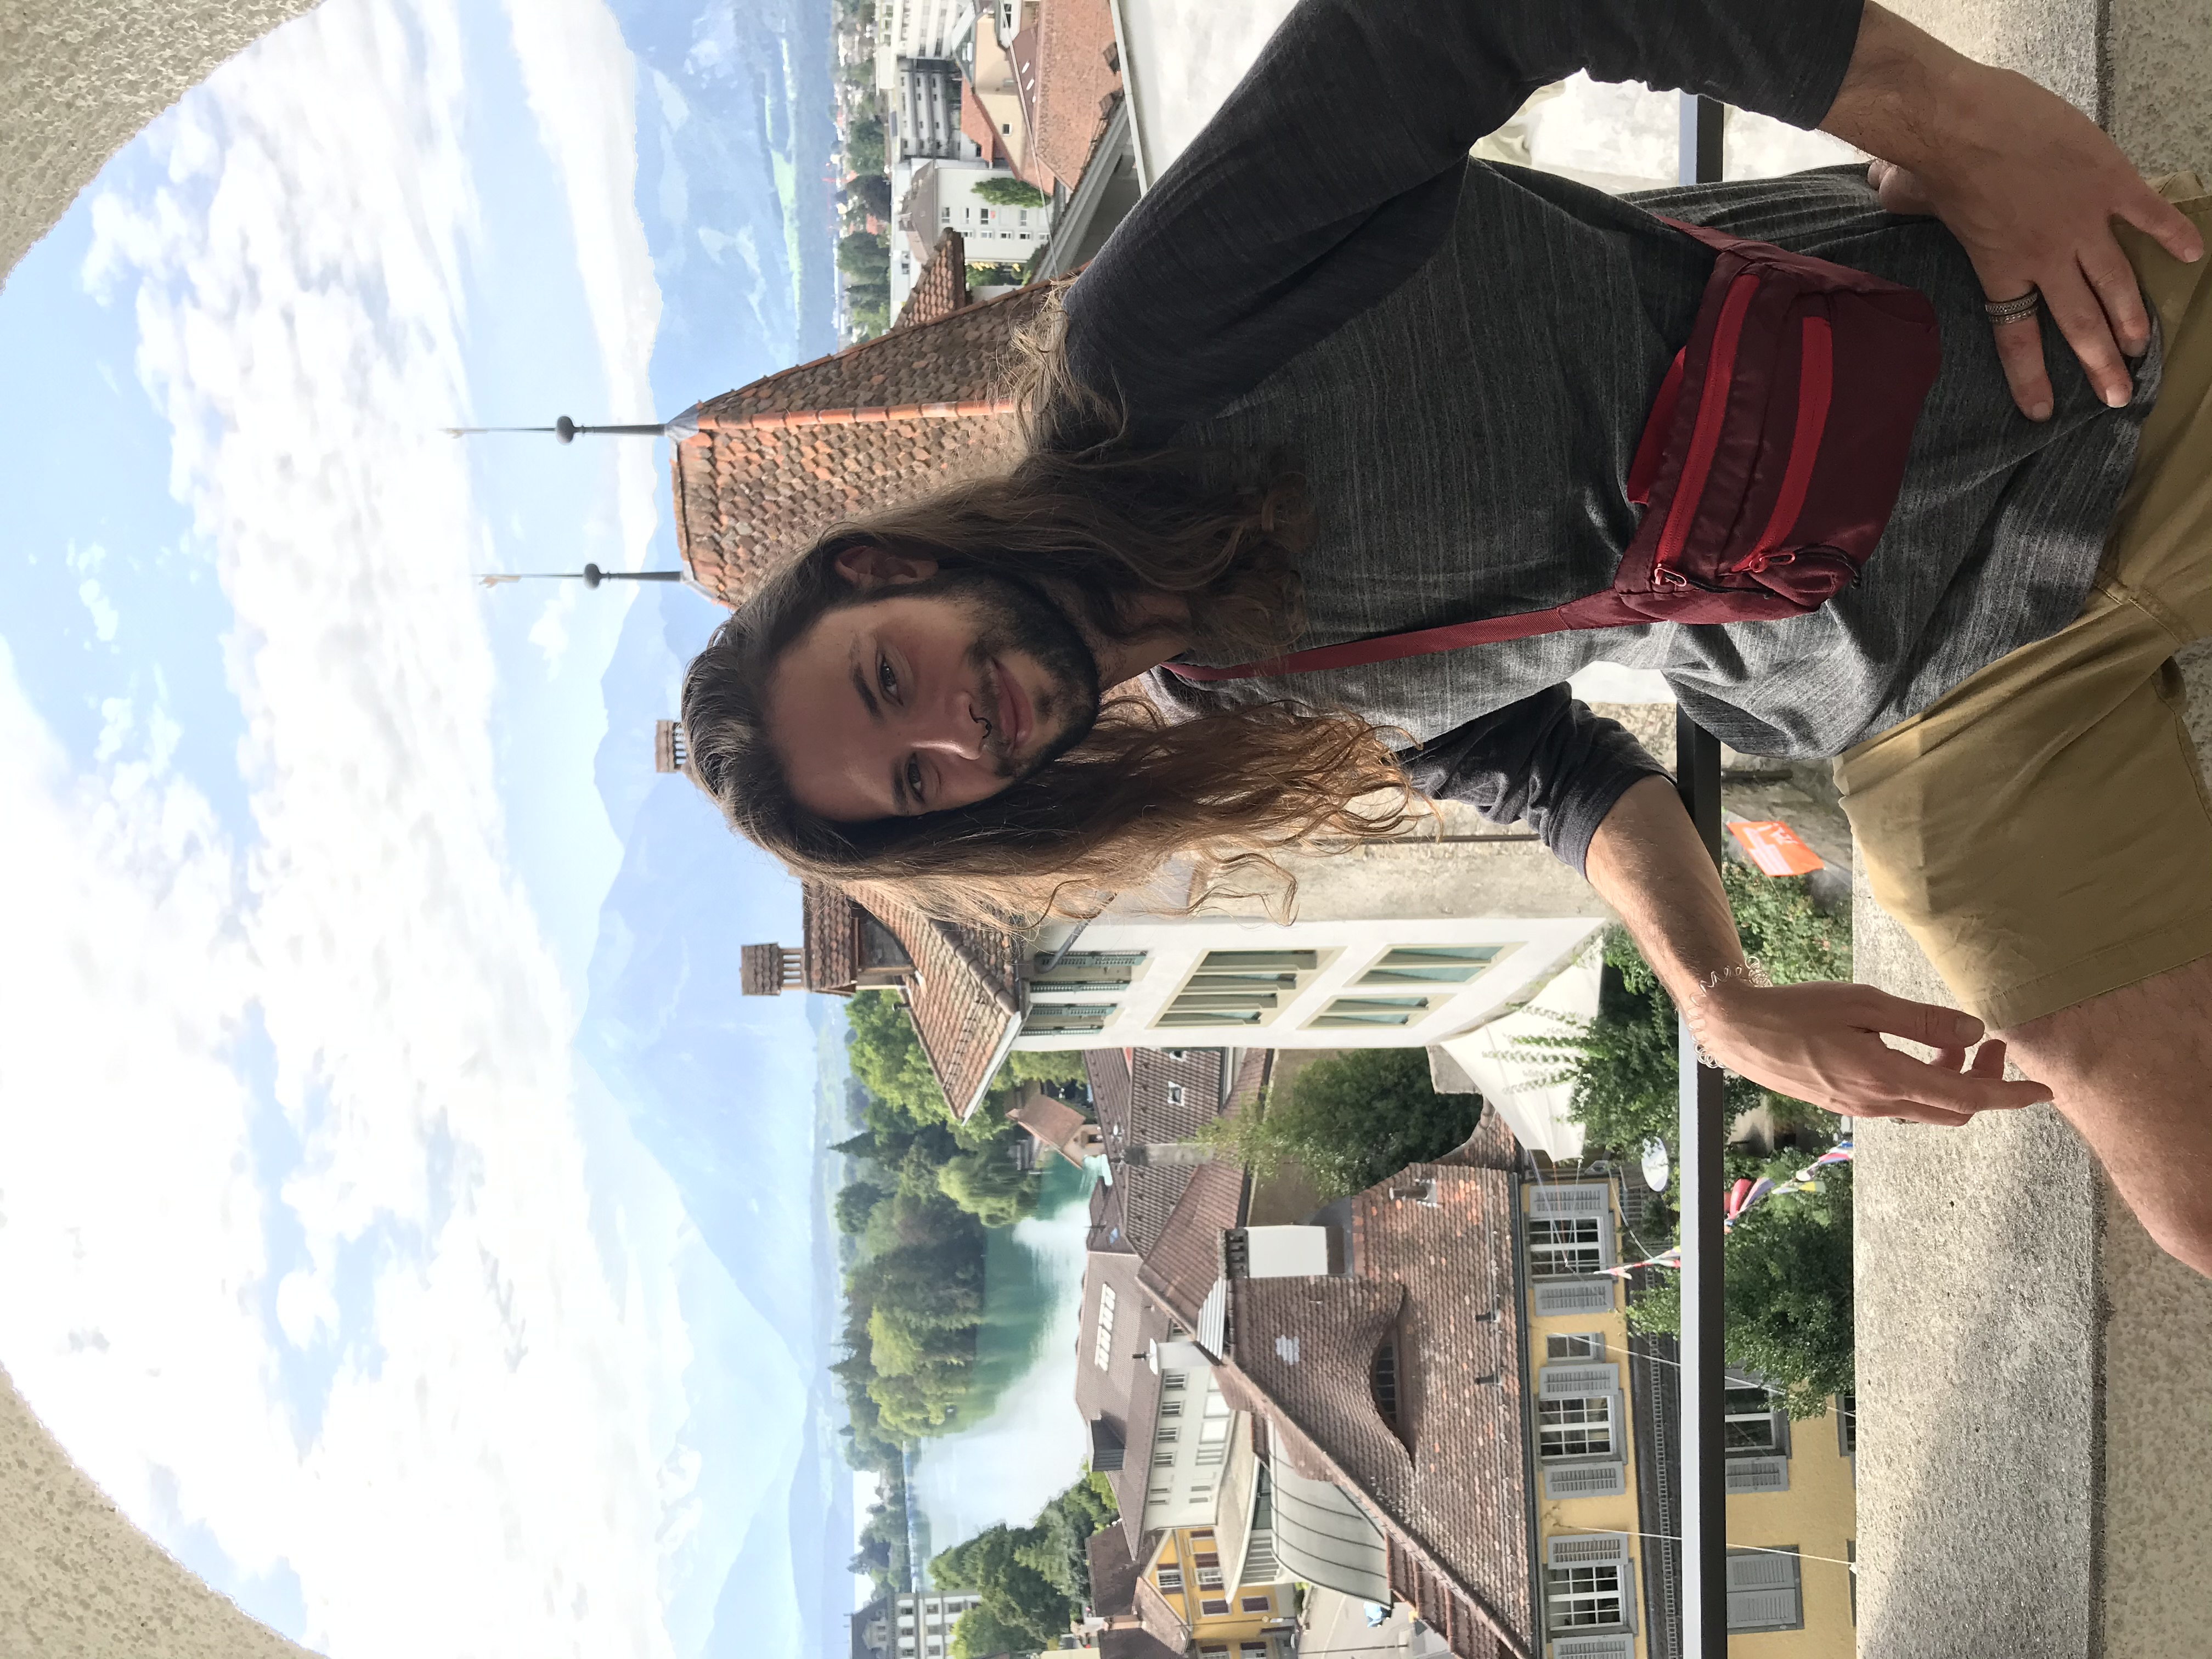
\includegraphics[angle=270,origin=c,width=3cm, height =5cm]{C:/Users/isaac/Pictures/Thun.jpg}
% use this format for absolute sizing
%\includegraphics[width=3cm, height=4cm]{filename.jpg}
\end{figure}
\end{frame}

% SLIDE (TABLE)----------------------------
\begin{frame}
\frametitle{Table}
\begin{table}
\begin{tabular}{l l l}
\toprule
\textbf{Treatments} & \textbf{Apple} & \textbf{Mango}\\
\midrule
Color & Red & Yellow \\
Weight & 390.1 g & 653.2 g \\
Taste & Crisp & Sweet \\
\bottomrule
\end{tabular}
\caption{Fruit is great!}
\end{table}
\end{frame}

% SLIDE (BLOCKS OF HIGHLIGHTED TEXT)-------
\begin{frame}
\frametitle{2 Truths and a Lie}
\begin{block}{Truth}
I gave an elderly woman the heimlich at work one day, while simultaneously having food poising. 
\end{block}

\begin{block}{Truth}
I have never been in any American time zone besides Eastern.
\end{block}

\begin{block}{Lie}
I love beets.
\end{block}
\end{frame}

% SLIDE (EMBEDDED R CODE)------------------
\begin{frame}[fragile]{Embedded R Code; \texttt{fragile} frame}
\begin{block}

\begin{knitrout}
\definecolor{shadecolor}{rgb}{0.969, 0.969, 0.969}\color{fgcolor}\begin{kframe}
\begin{alltt}
\hlcom{# show some output...}
\hlkwd{as.integer}\hlstd{(}\hlkwd{runif}\hlstd{(}\hlkwc{n}\hlstd{=}\hlnum{10}\hlstd{,} \hlkwc{min} \hlstd{=}\hlnum{1}\hlstd{,} \hlkwc{max} \hlstd{=}\hlnum{10}\hlstd{))}
\end{alltt}
\begin{verbatim}
##  [1] 6 3 5 2 6 9 8 2 8 3
\end{verbatim}
\end{kframe}
\end{knitrout}

\end{block}
\end{frame}

% SLIDE (EMBEDDED R FIGURE)----------------
\begin{frame}[fragile]{Embedded R Figure; \texttt{fragile} frame}
%\begin{block}

\begin{knitrout}
\definecolor{shadecolor}{rgb}{0.969, 0.969, 0.969}\color{fgcolor}

{\centering 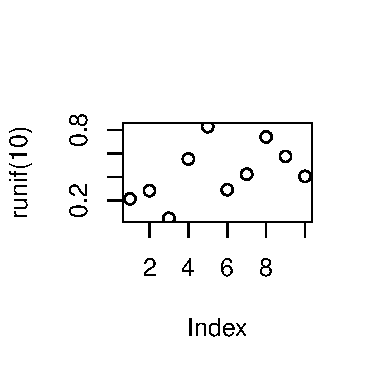
\includegraphics[width=\maxwidth]{figure/unnamed-chunk-2-1} 

}



\end{knitrout}

%\end{block}
\end{frame}


%Adding a comment to a plot---------------------
\begin{figure}
\centering
\begin{knitrout}
\definecolor{shadecolor}{rgb}{0.969, 0.969, 0.969}\color{fgcolor}\begin{figure}
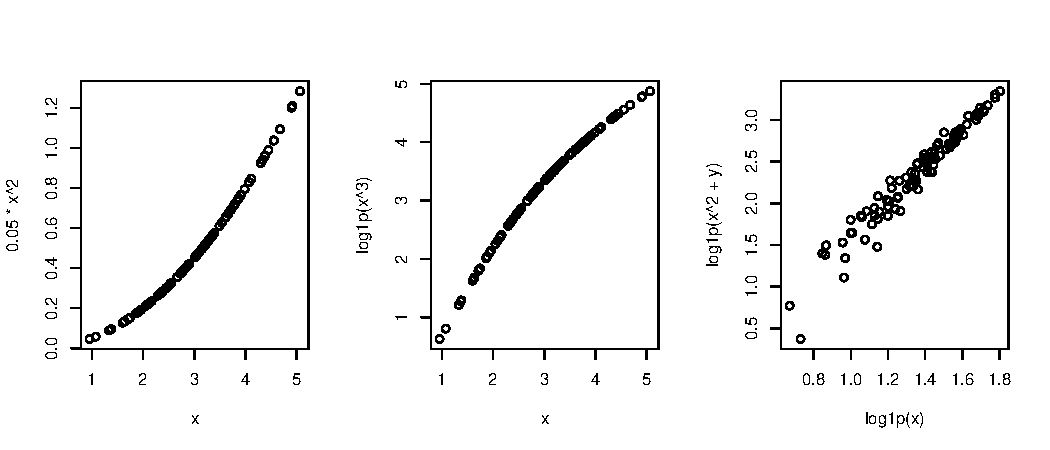
\includegraphics[width=\maxwidth]{figure/test-1} \caption[Three plots in one figure]{Three plots in one figure}\label{fig:test}
\end{figure}


\end{knitrout}
\caption{I got this example from tex.stackexchange from Fran!}
%credits: https://tex.stackexchange.com/questions/464843/caption-in-sweave-after-an-r-plot
\end{figure}


% SLIDE (MULTIPLE COLUMNS)-----------------
\begin{frame}
\frametitle{Multiple Columns}
\begin{columns}[c] % The "c" option specifies centered vertical alignment while the "t" option is used for top vertical alignment

\column{.45\textwidth} % Left column and width
\textbf{My likes}
\begin{enumerate}
\item Skiing
\item Traveling
\item Craft Beer
\item Vegetarian Cuisine
\end{enumerate}

\column{.5\textwidth} % Right column and width
I sure do have some expensive likes. Maybe I should go cross country skiing more and drink PBR to save up! Luckily, there are no chances to spend money on traveling right now. 

\end{columns}
\end{frame}


% SLIDE (THEOREM)----------------------------
\begin{frame}
\frametitle{Theorem}
\begin{theorem}[Electric Field Equation]
$E = K*q / r^2$
\end{theorem}
I really should study for physics more often.
\end{frame}


% SLIDE (FINAL SLIDE)------------------------
\begin{frame}
\Huge{\centerline{Fin}}
\end{frame}

%------------------------------------------------
\end{document}
